\documentclass[aspectratio=169]{beamer}

\usetheme{GRVC}

% -----------------------------
% Typography (keep blocks readable on 16:9)
% -----------------------------
\setbeamerfont{block title}{size=\normalsize, series=\bfseries}
\setbeamerfont{block body}{size=\small}
\setbeamerfont{itemize/enumerate body}{size=\small}
\setbeamerfont{itemize/enumerate subbody}{size=\footnotesize}

% -----------------------------
% Packages
% -----------------------------
\usepackage{tikz}
\usetikzlibrary{calc}
\usepackage{amsmath,amssymb}
\usepackage{mathtools}

% Allow figures to be placed either alongside this .tex file or inside an assets/ folder
\graphicspath{{./}{assets/}{assets/figures/}{figures/}}

% -----------------------------
% Math helpers
% -----------------------------
\DeclareMathOperator{\logit}{logit}
\DeclareMathOperator{\clip}{clip}

% Partner logo helper (used for consortium slides)
\newcommand{\GRVCpartnerlogo}[1]{%
  \includegraphics[width=0.16\textwidth,height=1.5cm,keepaspectratio]{#1}%
}

% Default background image for non-technical sections
\newcommand{\GRVCPhotoBackground}{%
  \setbeamertemplate{background}{%
    \begin{tikzpicture}[remember picture,overlay]
      \node[opacity=0.95, at=(current page.center)] {%
        \includegraphics[width=\paperwidth,height=\paperheight]{assets/background.png}%
      };
    \end{tikzpicture}%
  }%
}

% Clean solid background for equations / dense technical content (better legibility)
\newcommand{\GRVCSolidBackground}{%
  \setbeamertemplate{background}{%
    \begin{tikzpicture}[remember picture,overlay]
      \fill[GRVCBlue] (current page.south west) rectangle (current page.north east);
    \end{tikzpicture}%
  }%
}

\GRVCPhotoBackground

% -----------------------------
% Title meta
% -----------------------------
\title{GRVC Lab\\Biweekly seminars}
\author{Abdalraheem Abdullah Yousef Ijieh}
\date{16 Enero 2026}

\begin{document}

% ============================================================
% Title
% ============================================================
\begin{frame}[plain]
  \titlepage
\end{frame}

% ============================================================
% Roadmap (fixes pacing and expectations)
% ============================================================
\begin{frame}{Roadmap}
  \small
  \begin{enumerate}\itemsep0.5em
    \item TEMA context: partners and technologies (USE scope)
    \item PDM-tech-05: Information Fusion platform (problem \textrightarrow{} approach \textrightarrow{} outputs)
    \item Fusion methods: OGM (hazard occupancy) and OPM (multi-object tracking)
    \item Flood case study (Ahrtal): inputs, fusion evolution, outputs and lessons learned
  \end{enumerate}
\end{frame}

% ============================================================
% TEMA context
% ============================================================
\GRVCsectionframe[assets/tema\_logo.png]{Trusted extremely precise mapping and prediction for emergency management}

{
\GRVCsetprojectlogo{assets/tema_logo.pdf}

\begin{frame}{TEMA in a Nutshell}
  \begin{columns}[T,onlytextwidth]
    % ---------------- Left column: Partners ----------------
    \column{0.42\textwidth}
      \centering
      {\bfseries Consortium partners}\par\vspace{0.4em}

      \setlength{\tabcolsep}{3pt}
      \renewcommand{\arraystretch}{0.95}

      \begin{tabular}{ccccc}
        \GRVCpartnerlogo{assets/partners/auth.png} &
        \GRVCpartnerlogo{assets/partners/atos.png} &
        \GRVCpartnerlogo{assets/partners/brk.png} &
        \GRVCpartnerlogo{assets/partners/dmalian.png} &
        \GRVCpartnerlogo{assets/partners/engineering.png} \\
        \GRVCpartnerlogo{assets/partners/fraunhofer_hhi.png} &
        \GRVCpartnerlogo{assets/partners/dlr.png} &
        \GRVCpartnerlogo{assets/partners/itu.png} &
        \GRVCpartnerlogo{assets/partners/kamk.png} &
        \GRVCpartnerlogo{assets/partners/kaj.png} \\
        \GRVCpartnerlogo{assets/partners/kemea.png} &
        \GRVCpartnerlogo{assets/partners/latitudo40.png} &
        \GRVCpartnerlogo{assets/partners/nelen_schuurmans.png} &
        \GRVCpartnerlogo{assets/partners/northdocks.png} &
        \GRVCpartnerlogo{assets/partners/plus.png} \\
        \GRVCpartnerlogo{assets/partners/ras.png} &
        \GRVCpartnerlogo{assets/partners/tecnosylva.png} &
        \GRVCpartnerlogo{assets/partners/lisbon_council.png} &
        \GRVCpartnerlogo{assets/partners/use.png} &
        \GRVCpartnerlogo{assets/partners/unime.png} \\
      \end{tabular}

    % ---------------- Right column: At a glance ----------------
    \column{0.55\textwidth}
    \centering 
    {\bfseries \large TEMA at a glance}\par\vspace{0.3em}
    \centering
    \begin{tabular}{ccc}
      {20 Partners} & {4 Years} & {11 M\texteuro}
    \end{tabular}
    \par\vspace{0.6em}
    \raggedright

    \setbeamerfont{block title}{size=\footnotesize,series=\bfseries}
    \setbeamerfont{block body}{size=\scriptsize}
    \setbeamerfont{itemize/enumerate body}{size=\scriptsize}

    \begin{block}{Mission}
      Deliver actionable situational awareness for disaster response by turning multi-source data into decision-ready information.
    \end{block}

    \vspace{-0.3em}
    \begin{itemize}
      \setlength{\itemsep}{0.35em}
      \item Bring real-time situational data to responders and relevant end-users.
      \item Support operational decision-making during evolving incidents.
      \item Transferable across hazards (e.g., flood, wildfire) and geographic regions.
    \end{itemize}
  \end{columns}
\end{frame}
\GRVCclearprojectlogo
}

% ------------------------------------------------------------
% TEMA technologies (USE highlighted)
% ------------------------------------------------------------
{
\GRVCsetprojectlogo{assets/tema_logo.pdf}
\newcommand{\USEtech}[1]{\textbf{\textcolor{GRVCCyan}{#1}}}

\begin{frame}{TEMA technologies}
  \footnotesize
  \setlength{\tabcolsep}{2pt}
  \renewcommand{\arraystretch}{0.98}

  \begin{columns}[T,onlytextwidth]
    % ---------------- TFA ----------------
    \column{0.43\textwidth}
    {\bfseries Trustworthy Federated Analytics}\par\vspace{0.25em}
    \begin{tabular}{@{}p{0.25\linewidth}p{0.73\linewidth}@{}}
      \textbf{ID} & \textbf{Technology}\\ \hline
      TFA-tech-01 & Concept discovery for latent space interpretability of deep neural networks\\
      TFA-tech-02 & Human-comprehensible presentation of concept-based explanations\\
      TFA-tech-03 & DNN robustness\\
      TFA-tech-04 & Explainability for transformer base neural networks\\
      TFA-tech-05 & Fire/smoke/flood/person detection\\
      TFA-tech-06 & Fire/flood/background segmentation\\
      TFA-tech-07 & Person re-identification\\
      TFA-tech-08 & Satellite-based flood detection and assessment\\
      TFA-tech-09 & Satellite-based forest fire detection and assessment\\
      TFA-tech-10 & Privacy preservation during visual analysis\\
      TFA-tech-11 & Geo-social media analysis\\
      TFA-tech-12 & Sentiment analysis for short texts\\
      TFA-tech-13 & Contrastive image-language models\\
      TFA-tech-14 & Federated Learning\\
      TFA-tech-15 & Data scarcity, synthetic data generation pipeline\\
    \end{tabular}

    % ---------------- PDM ----------------
    \column{0.31\textwidth}
    {\bfseries Phenomenon Prediction and Decision-Making}\par\vspace{0.25em}
    \begin{tabular}{@{}p{0.45\linewidth}p{0.53\linewidth}@{}}
      \textbf{ID} & \textbf{Technology}\\ \hline
      PDM-tech-01 & Forest fire simulation\\
      PDM-tech-02 & 3Di hydrodynamic simulation\\
      PDM-tech-03 & Realistic 3D smoke modelling and fire detection\\
      \USEtech{PDM-tech-04} & \USEtech{Drone planning}\\
      \USEtech{PDM-tech-05} & \USEtech{Information fusion}\\
      PDM-tech-06 & Data-fusion-based decision support and process triggering\\
    \end{tabular}

    % ---------------- SV ----------------
    \column{0.25\textwidth}
    {\bfseries Simulation and Visualization}\par\vspace{0.25em}
    \begin{tabular}{@{}p{0.46\linewidth}p{0.52\linewidth}@{}}
      \textbf{ID} & \textbf{Technology}\\ \hline
      \USEtech{SV-tech-01} & \USEtech{Drone-based image and data acquisition}\\
      SV-tech-02 & Digital Enabler\\
      SV-tech-03 & 3D computer vision (SfM)/ Photogrammetry\\
      SV-tech-04 & Geovisual Analytics\\
      SV-tech-05 & Geospatial information retrieval\\
      SV-tech-06 & Extended Reality-based interactive visualisation system\\
      SV-tech-07 & SmartDesk\\
    \end{tabular}
  \end{columns}

  \vspace{0.4em}
  \scriptsize \textcolor{GRVCCyan}{\rule{0.9em}{0.9em}} \; \textit{University of Seville (USE): SV-tech-01, PDM-tech-04, PDM-tech-05.}
\end{frame}
\GRVCclearprojectlogo
}

% ============================================================
% Information Fusion (PDM-tech-05)
% ============================================================
\GRVCsectionframe[assets/tema\_logo.png]{Information fusion (PDM-tech-05)}

{
\GRVCsetprojectlogo{assets/tema_logo.pdf}
\GRVCSolidBackground

% -----------------------------
% Storyline
% -----------------------------
\begin{frame}{Information fusion: storyline}
  \small
  \begin{itemize}\itemsep0.45em
    \item Natural Disaster Management (NDM) produces many signals (UAV, satellite, models, geo-social), often \textbf{asynchronous} and sometimes \textbf{contradictory}.
    \item PDM-tech-05 turns these signals into a \textbf{single, continuously updated operational picture}.
    \item Two primary products:
      \begin{itemize}\itemsep0.25em
        \item \textbf{OGM (Occupancy Grid Map)}: disaster status as a probabilistic map (flood or fire).
        \item \textbf{OPM (Object Presence Map)}: tracked people/vehicles with uncertainty.
      \end{itemize}
    \item We validate the approach on a flood case study (Ahrtal), consistent with the draft paper.
  \end{itemize}
\end{frame}

\begin{frame}{Motivation: why we need information fusion}
  \begin{columns}[T,onlytextwidth]
    \column{0.58\textwidth}
      \small
      \begin{itemize}\itemsep0.55em
        \item In disasters, the bottleneck is not data availability, but \textbf{coherence}.
        \item UAV: detailed but local and intermittent.
        \item Satellite: wide-area but delayed and sometimes uncertain.
        \item Simulations: predictive but model-dependent.
        \item Geo-social: fast but noisy and biased.
      \end{itemize}
      \vspace{0.4em}
      \begin{block}{Goal}
        Provide one operational picture that updates whenever new evidence arrives.
      \end{block}
    \column{0.40\textwidth}
      \centering
      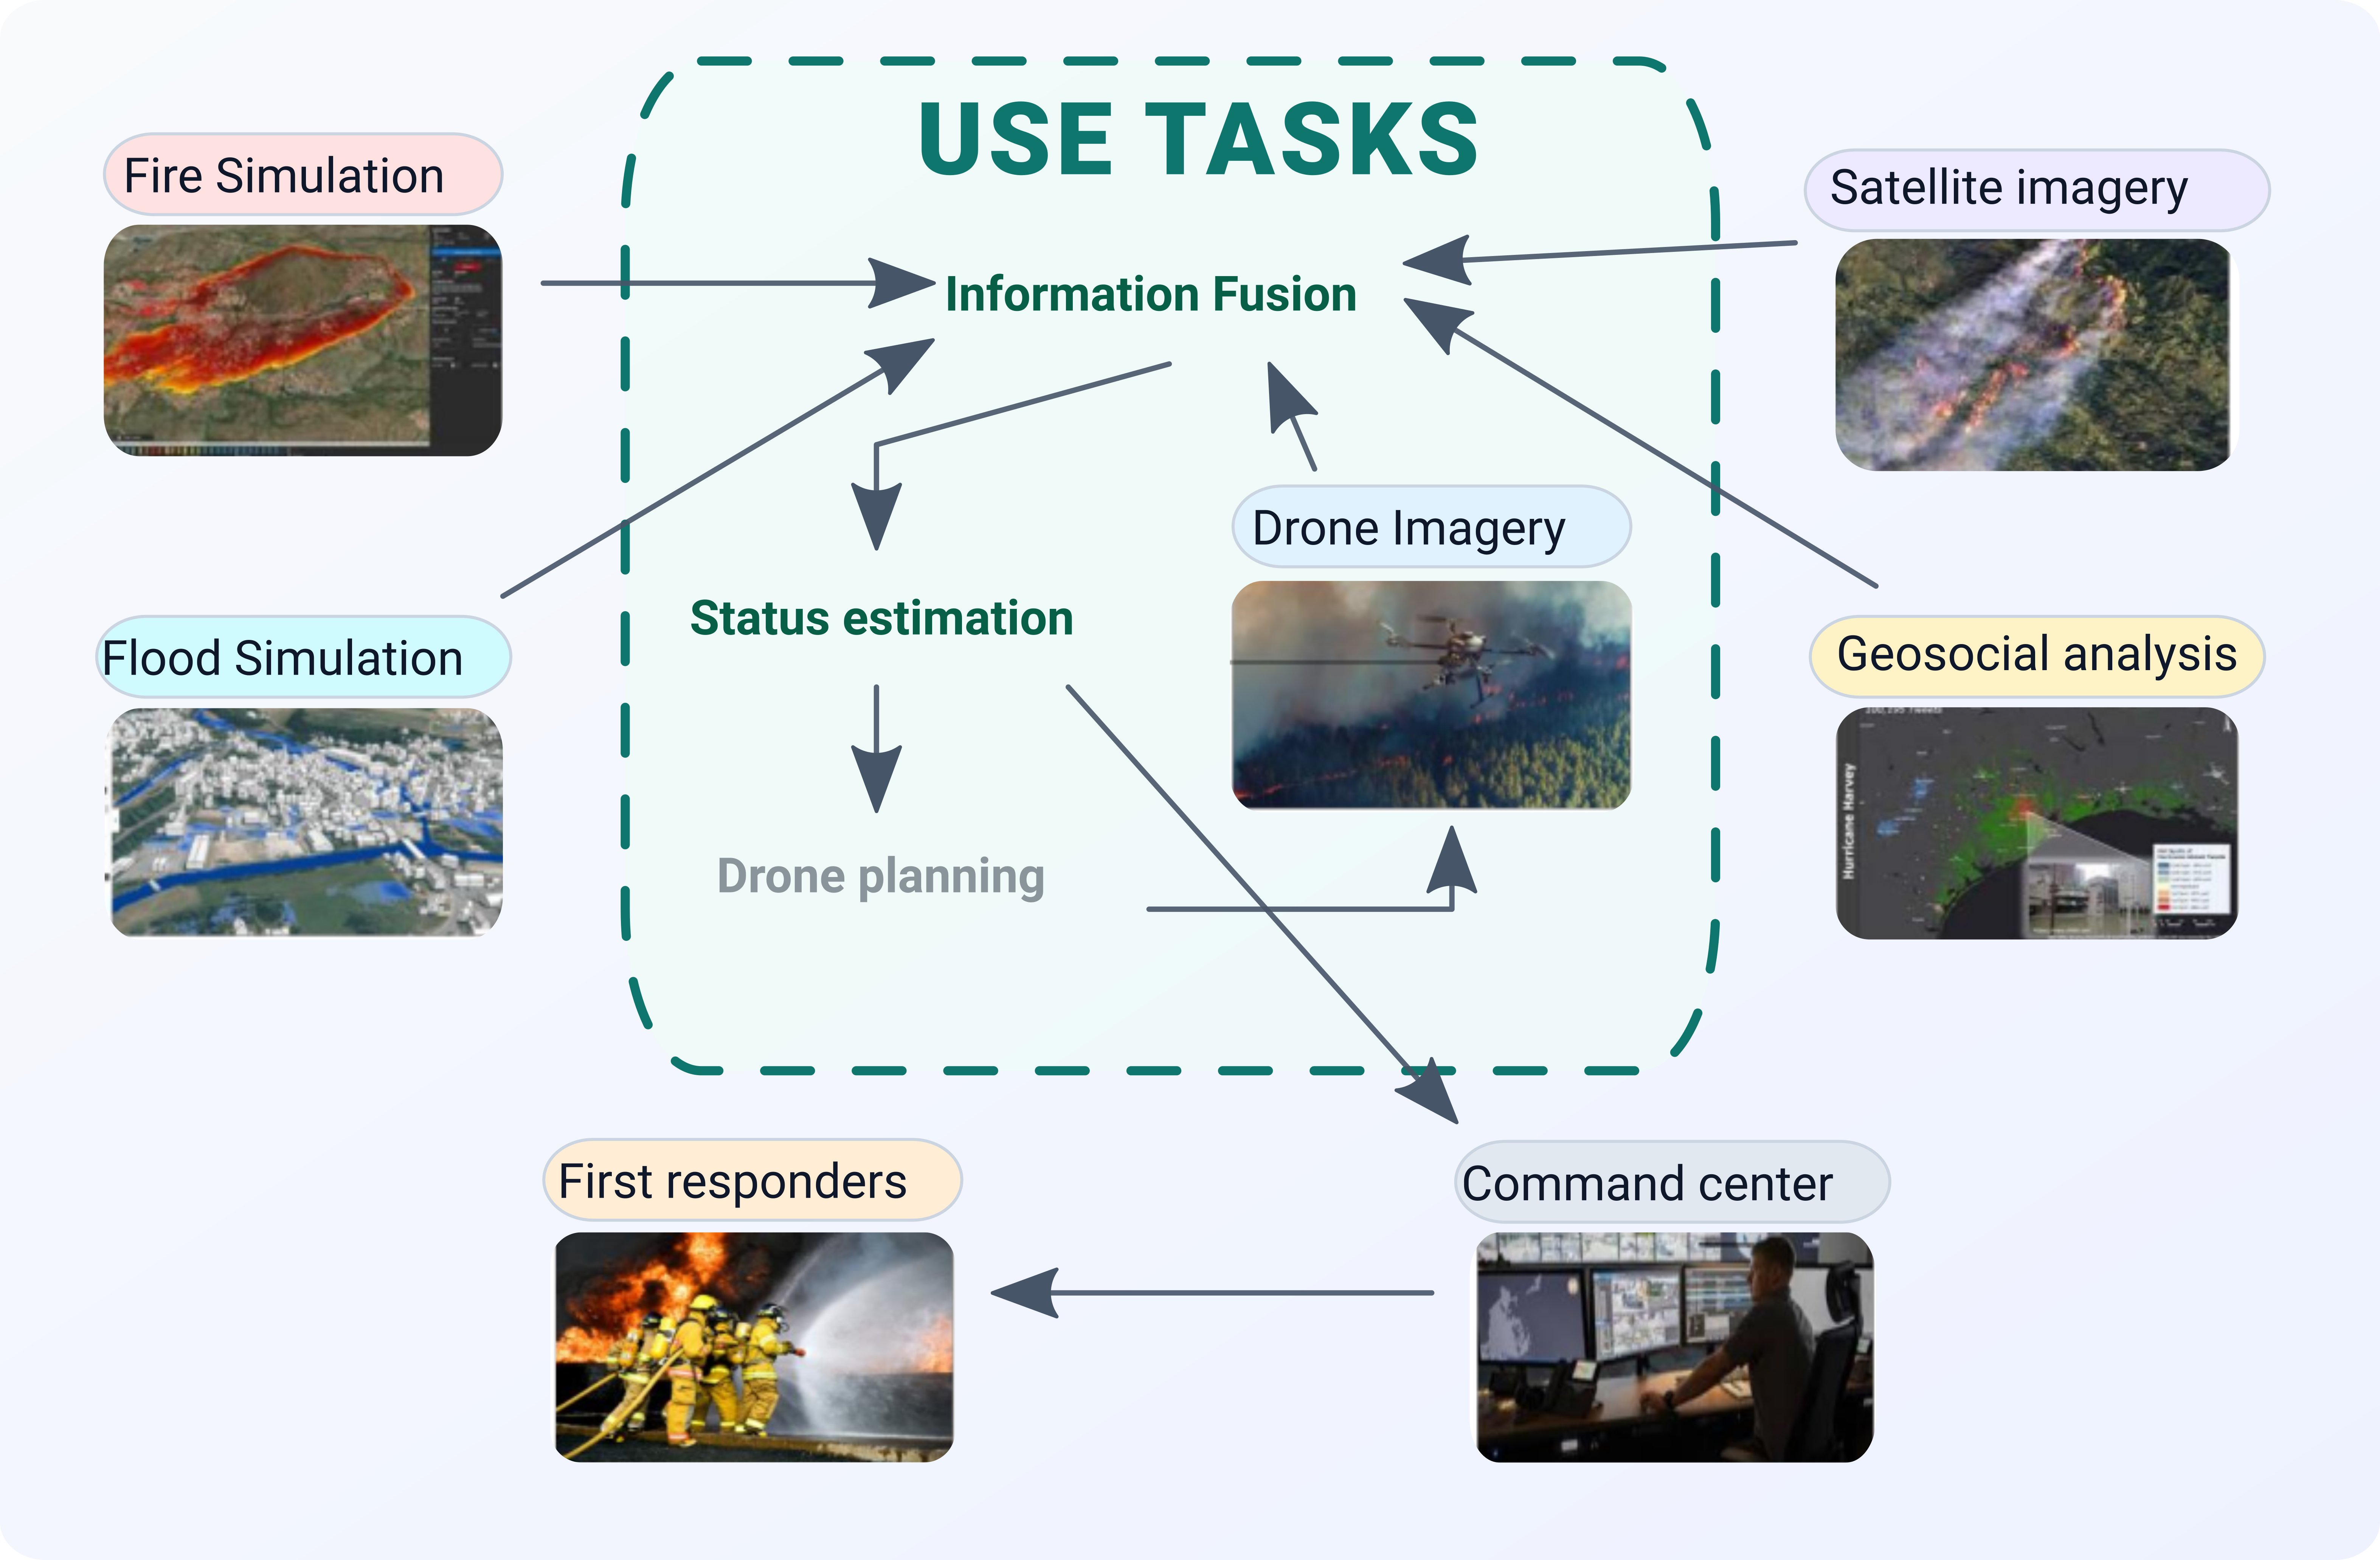
\includegraphics[width=\linewidth,height=0.72\textheight,keepaspectratio]{enhanced_end_to_end_scheme.png}
  \end{columns}
\end{frame}

\begin{frame}{Key challenges addressed by PDM-tech-05}
  \small
  \begin{itemize}\itemsep0.6em
    \item \textbf{Asynchrony:} different refresh rates and latencies (seconds to hours).
    \item \textbf{Heterogeneity:} masks, grids, point detections, text-derived signals, forecasts.
    \item \textbf{Uncertainty:} every source is imperfect; disagreement is normal.
    \item \textbf{Georeferencing:} mobile sensors + terrain \textrightarrow{} spatial alignment is non-trivial.
    \item \textbf{Dynamics:} evolving hazard fronts and moving objects \textrightarrow{} temporal consistency matters.
  \end{itemize}
\end{frame}

\begin{frame}{What the Information Fusion platform does}
  \begin{columns}[T,onlytextwidth]
    \column{0.53\textwidth}
      \small
      \begin{enumerate}\itemsep0.45em
        \item \textbf{Ingest} NGSI-LD entities (measurements + predictions).
        \item \textbf{Georeference} observations into a common map frame (AOI grid).
        \item \textbf{Fuse} evidence probabilistically (event-driven updates).
        \item \textbf{Track} objects over time (OPM).
        \item \textbf{Publish} updated products to SmartDesk and downstream services.
      \end{enumerate}
      \vspace{0.35em}
      \begin{block}{Platform property}
        Hazard-agnostic engine; hazard-specificity enters via input models and OGM semantics (Flood/Fire).
      \end{block}
    \column{0.45\textwidth}
      \centering
      \includegraphics[width=\linewidth,height=0.78\textheight,keepaspectratio]{INTERACTION_DIAGRAM.png}
  \end{columns}
\end{frame}

\begin{frame}{Web app and services architecture (deployment view)}
  \centering
  \includegraphics[width=\textwidth,height=0.86\textheight,keepaspectratio]{web_app_diagram.png}
\end{frame}

\begin{frame}{Core engine: asynchronous occupancy-grid mapping}
  \begin{columns}[T,onlytextwidth]
    \column{0.46\textwidth}
      \small
      \begin{itemize}\itemsep0.55em
        \item The OGM is updated \textbf{whenever} new evidence arrives.
        \item Measurements: update occupancy via inverse sensor models.
        \item Predictions: bias or propagate occupancy using forecast evidence.
        \item Asynchrony is handled naturally (no need to wait for all sources).
      \end{itemize}
    \column{0.52\textwidth}
      \centering
      \includegraphics[width=\linewidth,height=0.78\textheight,keepaspectratio]{asyncapproach.png}
  \end{columns}
\end{frame}

% ============================================================
% OGM equations (consistent log-odds formalism)
% ============================================================
\begin{frame}{OGM formalism: probability and log-odds}
  \scriptsize
  \setlength{\abovedisplayskip}{2pt}
  \setlength{\belowdisplayskip}{2pt}

  Discretize the AOI into cells $m_i$ and maintain an occupancy probability $p_t(i)=P(m_i \text{ occupied at time } t)$.
  \vspace{0.35em}

  \begin{align*}
    \ell_t(i) &= \log \frac{p_t(i)}{1-p_t(i)} \qquad\text{(log-odds)}\\
    p_t(i) &= \sigma(\ell_t(i))=\frac{1}{1+e^{-\ell_t(i)}} \qquad\text{(logistic)}\\
    \ell_0(i) &= \log \frac{P(m_i)}{1-P(m_i)} \qquad\text{(prior; often }P(m_i)=0.5\text{)}
  \end{align*}

  \begin{block}{Why log-odds?}
    Numerical stability and additive updates across asynchronous sources.
  \end{block}
\end{frame}

\begin{frame}{OGM fusion rule: Bayesian update in log-odds}
  \scriptsize
  \setlength{\abovedisplayskip}{2pt}
  \setlength{\belowdisplayskip}{2pt}

  For an incoming observation $z_t$ (from any source) and platform state $x_t$:
  \begin{align*}
    \ell_t(i)
    &= \ell_{t^-}(i) + \underbrace{\logit\!\big(P(m_i \mid z_t,x_t)\big)}_{\text{source evidence}} - \ell_0(i)
  \end{align*}

  \begin{block}{Interpretation}
    Each source produces a per-cell occupancy probability; we convert it to a log-odds increment and add it to the current map (subtracting the prior once to avoid double counting).
  \end{block}
\end{frame}

\begin{frame}{Fusion of measurements vs.\ predictions}
  \small
  \begin{itemize}\itemsep0.6em
    \item \textbf{Measurements} (UAV/satellite/geo-social) update the current OGM via inverse sensor models.
    \item \textbf{Predictions} (e.g., hydrodynamics, fire simulation) encode forecast evidence and are fused conservatively:
      \begin{itemize}\itemsep0.3em
        \item as log-odds evidence, or
        \item via \textbf{logit pooling} (weighted fusion in log-odds space).
      \end{itemize}
    \item The platform remains generic: source-specificity enters only through the mapping from raw outputs to $p^{(s)}_t(i)$.
  \end{itemize}
\end{frame}

% ============================================================
% Flood measurement models (examples)
% ============================================================
\begin{frame}{Flood measurement model: UAV flood segmentation (TFA-tech-06)}
  \tiny
  \setlength{\abovedisplayskip}{1pt}
  \setlength{\belowdisplayskip}{1pt}

  Segmentation provides per-pixel flood scores $s_k^{uav}\in[0,1]$ for UAV pixels $k$ projected into grid cell $i$.

  \begin{align*}
    \bar{s}^{uav}_i &= \frac{1}{n_i}\sum_{k \in K_i} s^{uav}_k \\
    p^{uav}_i &= p^{uav}_{\min} + \left(p^{uav}_{\max}-p^{uav}_{\min}\right)\bar{s}^{uav}_i \\
    \delta\ell^{uav}(i) &= \logit(p^{uav}_i) - \ell_0(i), \qquad \ell_t(i)=\ell_{t^-}(i)+\delta\ell^{uav}(i)
  \end{align*}

  \begin{block}{Notes}
    $p^{uav}_{\min},p^{uav}_{\max}$ encode trust in the segmentation (avoid overconfidence).
  \end{block}
\end{frame}

\begin{frame}{Flood measurement model: satellite flood extent (TFA-tech-08)}
  \tiny
  \setlength{\abovedisplayskip}{1pt}
  \setlength{\belowdisplayskip}{1pt}

  Satellite products provide a per-cell probability (or a mask mapped to probability) $m^{sat}_i\in[0,1]$.

  \begin{align*}
    p^{sat}_i &= \clip\!\left(m^{sat}_i,\varepsilon,1-\varepsilon\right)\\
    \delta\ell^{sat}(i) &= \logit(p^{sat}_i) - \ell_0(i), \qquad \ell_t(i)=\ell_{t^-}(i)+\delta\ell^{sat}(i)
  \end{align*}

  \begin{block}{Notes}
    $\varepsilon$ prevents infinite log-odds; confidence can be source-dependent (clouds, resolution, latency).
  \end{block}
\end{frame}

\begin{frame}{Flood measurement model: geo-social hotspots (TFA-tech-11)}
  \tiny
  \setlength{\abovedisplayskip}{1pt}
  \setlength{\belowdisplayskip}{1pt}

  Geo-social analytics yields a spatial score from activity and relevance signals (normalized per AOI):
  \begin{align*}
    s^{soc}_t(i) &= w_c\,\tilde{c}_t(i) + w_r\,\tilde{r}_t(i), \qquad w_c+w_r=1 \\
    p^{soc}_t(i) &= \varepsilon + (1-2\varepsilon)\, s^{soc}_t(i) \\
    \delta\ell^{soc}(i) &= \logit(p^{soc}_t(i)) - \ell_0(i), \qquad \ell_t(i)=\ell_{t^-}(i)+\delta\ell^{soc}(i)
  \end{align*}

  \begin{block}{Notes}
    Geo-social is treated as uncertain evidence (conservative bounds and weights).
  \end{block}
\end{frame}

% ============================================================
% Flood prediction fusion (3Di example)
% ============================================================
\begin{frame}{Flood prediction fusion: hydrodynamic depth (PDM-tech-02 / 3Di)}
  \tiny
  \setlength{\abovedisplayskip}{1pt}
  \setlength{\belowdisplayskip}{1pt}

  Convert predicted water depth $h_i$ into occupancy probability via a logistic mapping:
  \begin{align*}
    p^{hyd}_i &= \varepsilon + (1-2\varepsilon)\,\frac{1}{1+\exp\left(-\frac{h_i-h_{50}}{s}\right)} \\
    \ell^{hyd}_i &= \logit(p^{hyd}_i)
  \end{align*}

  \textbf{Logit pooling (weighted fusion in log-odds space):}
  \begin{align*}
    \ell^{new}_i &= (1-\alpha_{hyd})\,\ell^{ogm}_i + \alpha_{hyd}\,\ell^{hyd}_i, \qquad p^{new}_i=\sigma(\ell^{new}_i)
  \end{align*}

  \begin{block}{Notes}
    $\alpha_{hyd}\in[0,1]$ controls reliance on prediction vs.\ accumulated evidence.
  \end{block}
\end{frame}

\begin{frame}{Extending beyond floods: fire occupancy (Maps4Fire)}
  \small
  \begin{itemize}\itemsep0.6em
    \item Same OGM formalism; semantics change to fire/smoke/burnt area occupancy.
    \item Example: combine active-fire and burnt-area evidence:
      \[
        p_m(i)=w_{fire}\,p_{fire}(i)+w_{burnt}\,p_{burnt}(i),\qquad w_{fire}+w_{burnt}=1
      \]
    \item Update $\ell_t(i)$ using the same log-odds update / pooling rules.
  \end{itemize}
\end{frame}

% ============================================================
% OPM: tracking (multi-object)
% ============================================================
\begin{frame}{OPM: state, motion model, and prediction}
  \scriptsize
  \setlength{\abovedisplayskip}{2pt}
  \setlength{\belowdisplayskip}{2pt}

  Track $k$ maintains a 6D state (geodetic position + velocity):
  \[
    x_{t,k}=\begin{bmatrix}\lambda&\phi&h&\dot{\lambda}&\dot{\phi}&\dot{h}\end{bmatrix}^{\!\top}
  \]

  Constant-velocity transition:
  \[
    x_{t+1,k}=A x_{t,k} + w_t,\quad
    A=\begin{bmatrix}
      1&0&0&\Delta t&0&0\\
      0&1&0&0&\Delta t&0\\
      0&0&1&0&0&\Delta t\\
      0&0&0&1&0&0\\
      0&0&0&0&1&0\\
      0&0&0&0&0&1
    \end{bmatrix}
  \]

  Prediction step:
  \[
    \hat{x}_{t|t-1,k}=A\hat{x}_{t-1|t-1,k},\qquad
    P_{t|t-1,k}=AP_{t-1|t-1,k}A^\top+Q
  \]
\end{frame}

\begin{frame}{OPM data association: gating and Hungarian assignment}
  \scriptsize
  \setlength{\abovedisplayskip}{2pt}
  \setlength{\belowdisplayskip}{2pt}

  For detection $j$ at position $p_{t,j}$ and predicted track position $\hat{p}_{t|t-1,k}$:
  \[
    d_{k,j}=d_{hav}(\hat{p}_{t|t-1,k},p_{t,j})
  \]

  Cost matrix for assignment (example):
  \[
    C_{k,j}=\alpha\,\frac{d_{k,j}}{r_{gate}}+\beta\,(1-c^{det}_{t,j})
  \]

  \begin{block}{Association}
    Apply gating ($d_{k,j}<r_{gate}$) then solve the assignment with the Hungarian algorithm.
  \end{block}
\end{frame}

\begin{frame}{OPM state correction: confidence-aware Kalman update}
  \scriptsize
  \setlength{\abovedisplayskip}{2pt}
  \setlength{\belowdisplayskip}{2pt}

  Measurement model (position):
  \[
    z_{t,j}=H x_{t,k}+v_t,\quad
    H=\begin{bmatrix}1&0&0&0&0&0\\0&1&0&0&0&0\\0&0&1&0&0&0\end{bmatrix}
  \]

  Confidence-aware measurement noise:
  \[
    R_{t,j}=\frac{1}{\max(c^{det}_{t,j},\varepsilon_c)}\,R_{base}
  \]

  Kalman update:
  \[
    S=HPH^\top+R,\quad K=PH^\top S^{-1},\quad
    \hat{x}_{t|t}=\hat{x}_{t|t-1}+K(z-H\hat{x}_{t|t-1})
  \]
\end{frame}

% ============================================================
% Case study: Ahrtal floods (detailed)
% ============================================================
\GRVCsectionframe[assets/tema\_logo.png]{Case study: Ahrtal floods}

\begin{frame}{Case study setup: AOI and common grid}
  \begin{columns}[T,onlytextwidth]
    \column{0.55\textwidth}
      \small
      \begin{itemize}\itemsep0.55em
        \item AOI defined as a polygon; discretized into an OGM grid.
        \item Initialization: $p_0(i)=0.5$ (unknown) inside AOI.
        \item Asynchronous fusion as sources arrive: 3Di prediction, UAV segmentation, satellite extent, geo-social hotspots.
        \item Objective: progressively refine the flood probability map (FPM).
      \end{itemize}
    \column{0.43\textwidth}
      \centering
      \includegraphics[width=\linewidth,height=0.75\textheight,keepaspectratio]{assets/aoi_satellite_with_bw_colorbar.png}
  \end{columns}
\end{frame}

\begin{frame}{Asynchronous inputs: what arrives, and when}
  \small
  \begin{columns}[T,onlytextwidth]
    \column{0.56\textwidth}
      \begin{itemize}\itemsep0.55em
        \item Case study is driven by event arrivals, not a fixed fusion cycle.
        \item Predictions provide early structure; observations correct local errors and sharpen boundaries.
        \item Practical implication: the operational picture improves continuously, without waiting for a ``complete'' dataset.
      \end{itemize}
    \column{0.42\textwidth}
      \centering
      \includegraphics[width=\linewidth,height=0.72\textheight,keepaspectratio]{assets/measurement_availability.png}
  \end{columns}
\end{frame}

\begin{frame}{3Di prediction: depth $\rightarrow$ flood probability prior}
  \begin{columns}[T,onlytextwidth]
    \column{0.48\textwidth}
      \centering
      \includegraphics[width=\linewidth,height=0.72\textheight,keepaspectratio]{assets/3di_depth.png}
      \vspace{0.3em}
      \scriptsize Predicted water depth (3Di)
    \column{0.48\textwidth}
      \centering
      \includegraphics[width=\linewidth,height=0.72\textheight,keepaspectratio]{assets/3di_probability.png}
      \vspace{0.3em}
      \scriptsize Mapped flood probability $p^{hyd}_i$
  \end{columns}
  \vspace{0.2em}
  \footnotesize
  \begin{itemize}\itemsep0.25em
    \item Prediction is fused conservatively (logit pooling) to avoid over-committing early.
    \item Sets the initial large-scale structure before high-resolution observations arrive.
  \end{itemize}
\end{frame}

\begin{frame}{UAV flood segmentation: image $\rightarrow$ mask $\rightarrow$ georeferenced evidence}
  \centering
  % --- Top row: three-stage visual narrative ---
  \includegraphics[width=0.32\linewidth,height=0.30\textheight,keepaspectratio]{assets/uav_captured_img.jpg}\hfill
  \includegraphics[width=0.32\linewidth,height=0.30\textheight,keepaspectratio]{assets/Flood_DJI_20211023131552_0001_Z_A.jpg}\hfill
  \includegraphics[width=0.32\linewidth,height=0.30\textheight,keepaspectratio]{assets/uav_geotiff_on_satellite.jpg}

  \vspace{0.35em}
  \begin{columns}[T,onlytextwidth]
    \column{0.56\textwidth}
      \small
      \begin{itemize}\itemsep0.4em
        \item UAV RGB imagery segmented into flood / non-flood.
        \item Mask is \textbf{georeferenced} onto the AOI (pose + DEM).
        \item Produces local, high-resolution observational evidence to correct the map.
      \end{itemize}
    \column{0.42\textwidth}
      \centering
      \includegraphics[width=\linewidth,height=0.40\textheight,keepaspectratio]{assets/uav_segmentation.png}
  \end{columns}
\end{frame}

\begin{frame}{Satellite flood extent: wide-area observational update}
  \begin{columns}[T,onlytextwidth]
    \column{0.52\textwidth}
      \small
      \begin{itemize}\itemsep0.5em
        \item Provides broader coverage than UAV but typically with latency.
        \item Converts extent/score into per-cell likelihood $p^{sat}_i$.
        \item Used to correct large-scale misalignment and fill gaps outside UAV footprint.
      \end{itemize}
    \column{0.46\textwidth}
      \centering
      \includegraphics[width=\linewidth,height=0.75\textheight,keepaspectratio]{assets/satellite_aoi.png}
  \end{columns}
\end{frame}

\begin{frame}{Geo-social hotspots: human-centric evidence (and limitations)}
  \begin{columns}[T,onlytextwidth]
    \column{0.46\textwidth}
      \small
      \begin{itemize}\itemsep0.45em
        \item Posts aggregated into hotspot cells (counts, activity, statistics).
        \item Converted into a measurement likelihood $p^{soc}_t(i)$.
        \item Ahrtal limitation: AOI falls mainly in a \textbf{single hotspot cell} \textrightarrow{} coarse spatial signal.
      \end{itemize}
    \column{0.52\textwidth}
      \centering
      \includegraphics[width=\linewidth,height=0.34\textheight,keepaspectratio]{assets/geosocial_raw.png}\\[0.35em]
      \includegraphics[width=\linewidth,height=0.34\textheight,keepaspectratio]{assets/geosocial_pm.png}
  \end{columns}
\end{frame}

\begin{frame}{Qualitative evolution: the FPM sharpens as evidence arrives}
  \centering
  \setlength{\tabcolsep}{3pt}
  \renewcommand{\arraystretch}{1.0}
  \begin{tabular}{cc}
    \includegraphics[width=0.48\linewidth,height=0.33\textheight,keepaspectratio]{assets/fpm_after_3di_greys_inset.png} &
    \includegraphics[width=0.48\linewidth,height=0.33\textheight,keepaspectratio]{assets/fpm_before_geosocial_zoom_cells.png} \\
    \includegraphics[width=0.48\linewidth,height=0.33\textheight,keepaspectratio]{assets/fpm_after_geosocial_zoom_cells.png} &
    \includegraphics[width=0.48\linewidth,height=0.33\textheight,keepaspectratio]{assets/final_fpm_multimodal_fusion.png}
  \end{tabular}

  \vspace{0.35em}
  \footnotesize
  \begin{itemize}\itemsep0.25em
    \item Prediction provides early structure; observations refine boundaries and correct local mismatches.
    \item Geo-social contribution is deliberately moderate but visible in the inset where applicable.
  \end{itemize}
\end{frame}

\begin{frame}{Quantitative evolution: uncertainty reduction and change detection}
  \begin{columns}[T,onlytextwidth]
    \column{0.54\textwidth}
      \small
      \begin{itemize}\itemsep0.6em
        \item Track the entropy of the flood probability map (FPM) to quantify confidence gains.
        \item Use map-to-map changes ($\Delta$) to detect when new evidence meaningfully updates the picture.
        \item In Ahrtal, the strongest corrections coincide with UAV and satellite arrivals.
      \end{itemize}
    \column{0.44\textwidth}
      \centering
      \includegraphics[width=\linewidth,height=0.75\textheight,keepaspectratio]{assets/fpm_entropy_delta.png}
  \end{columns}
\end{frame}

\begin{frame}{OPM case-study snapshot: tracking outputs}
  \begin{columns}[T,onlytextwidth]
    \column{0.55\textwidth}
      \small
      \begin{itemize}\itemsep0.55em
        \item OPM produces stable trajectories rather than flickering detections.
        \item Prediction fills gaps; corrections refine positions when detections arrive.
        \item Confidence-aware updates reduce overreaction to low-quality detections.
      \end{itemize}
    \column{0.43\textwidth}
      \centering
      \includegraphics[width=\linewidth,height=0.75\textheight,keepaspectratio]{assets/4_longitude_over_time.png}
  \end{columns}
\end{frame}

% ============================================================
% Wrap-up
% ============================================================
\begin{frame}{Key takeaways}
  \small
  \begin{itemize}\itemsep0.6em
    \item \textbf{Generic platform} for NDM: consistent handling of heterogeneous, asynchronous evidence.
    \item \textbf{Two operational products:} OGM (Flood/Fire status) and OPM (multi-object tracking).
    \item \textbf{Robust fusion:} Bayesian log-odds updates for measurements + logit pooling for predictions.
    \item \textbf{Operationalization:} event-driven services + web app cockpit + NGSI-LD interoperability.
    \item \textbf{USE loop:} Fusion $\rightarrow$ Drone planning $\rightarrow$ Drone acquisition $\rightarrow$ Fusion.
  \end{itemize}
\end{frame}

\begin{frame}{Q\&A}
  \centering
  \Large Questions?
\end{frame}

\GRVCclearprojectlogo
} % end Information Fusion group (restores global background)

\end{document}
